%!TEX root = ../../adrien_gomar_phd.tex

\chapter*{Conclusion}

The present PhD thesis aims at applying the Harmonic Balance (HB) approach to the 
aeroelasticity of a new type of aircraft engine: 
the Contra-Rotating Open Rotor (CROR). The method is 
first validated on analytical and linear and non-linear 
numerical test problems in \hyperref[cha:validation_hb]{\emph{Chapter~4}}. 
Two issues are raised, which prevent the use of such an approach 
on arbitrary aeroelastic configurations: the conditioning of
the multi-frequential HB source term and the
convergence of the method. Original methodologies are developed 
to improve the condition number of the simulations 
(\hyperref[cha:limitations_condition_number]{\emph{Chapter~5}})
and to provide a priori estimates of the number of harmonics 
required to achieve a given convergence level
(\hyperref[cha:limitations_convergence]{\emph{Chapter~6}}). 
The HB method is then validated for a standard configuration 
for turbomachinery aeroelasticity in \hyperref[cha:stcf11]{\emph{Chapter~7}}. 
The results are shown to be in good agreement 
with the experimental data. The applicability of the method 
is finally demonstrated for aeroelastic 
simulations of CROR
in \hyperref[cha:dream_ls_isolated]{\emph{Chapter~8}}
and \hyperref[cha:dream_hs_isolated]{\emph{Chapter~9}}.

\section*{Summary of the results}

\subsection*{On the conditioning of multi-frequential harmonic balance methods}

When the considered unsteadiness is related to a single frequency and its
harmonics (\emph{i.e.} the signal is periodic), 
Fourier analysis leads to a natural choice for the time instances
needed to compute the source term:
they are evenly spaced over the period. In this case, the mathematical
problem is numerically well-defined, meaning that the conditioning of
the operators ensures the convergence of the approach.
In opposite, when several arbitrary frequencies are 
considered (\emph{i.e.} the signal is almost periodic), as for instance CROR
aeroelasticity, the multi-frequential HB approach
is required and its source term can be ill-conditioned.

In \hyperref[cha:limitations_condition_number]{\emph{Chapter~5}},
we demonstrated that the time sampling has a major effect on the
stability of the multi-frequential HB 
method, due to the condition number of the discrete Fourier
transform matrix. One way to tackle this issue, 
is to consider a non-uniform time sampling
along with an algorithm to properly choose the time instances
as proposed by \citet{ThesisGuedeney}.
The Almost-Periodic Fourier Transform algorithm (APFT) 
algorithm, originally developed by \citet{Kundert1988} and implemented by 
\citet{ThesisGuedeney}, is shown to improve the discrete
Fourier transform matrix condition number.
However, for segregated frequencies, this condition number
is shown to remain too large to be used within an industrial context.

As the aeroelasticity of CROR is by essence
composed of segregated frequencies, new algorithms are needed.
This is why, a gradient-based OPTimization algorithm (OPT) 
has been developed in the current work.
It directly minimizes the condition number thanks to a
gradient-based optimization method. This last has proved to
give a condition number that is almost unity (\emph{i.e.} the
theoretical lower bound) for any input frequencies,
thus alleviating the stability issues encountered for arbitrary
multi-frequential HB computations.
This is a pre-processing procedure
that takes less than a minute.
Therefore, the non-uniform time sampling proposed by \citet{ThesisGuedeney}
used together with the OPT algorithm 
developed in the present contribution
enables to tackle problems with large frequency 
separation or large unsteadinesses, namely CROR aeroelasticity
can be considered.
This work has been published in
\begin{quote}
	\citetalias{JGuedeney2013}
\end{quote}


\subsection*{On the convergence of Fourier-based time methods}

Efficiency of Fourier-based time methods results 
from a trade-off between accuracy and 
costs requirements.
On one hand, the accuracy depends on the number of harmonics
used to represent the frequency content of the time 
signal; on the other hand, computational costs and 
memory consumption of the computations also scale
with the number of harmonics. 
The problem is that this number is 
configuration-dependent and hardly predictable. 
Moreover, a high number of harmonics
($\geq 10$) can prevent the use of such an approach,
as it might be more expensive than a classical time-marching approach.
This is particularly true on CROR configurations where the number
of harmonics needed to reach convergence
has been shown to be greater than ten
on some configurations~\cite{ThesisFrancois}.

In \hyperref[cha:limitations_convergence]{\emph{Chapter~6}}
we investigated the accuracy and convergence properties 
of Fourier-based time methods. It is highlighted that the convergence rate 
of these methods, in terms of harmonics required to describe the solution 
with a given level of accuracy, depends on the spectral content of the 
solution itself: Fourier-based time methods are particularly efficient 
for flow problems characterized by a narrow Fourier 
spectrum. 

We showed that the main source of unsteadiness in 
turbomachinery flows is due to the relative motion of wakes 
generated by a given blade row with respect to the downstream row.
\citet{Lakshminarayana1980} showed that the wake
behind turbomachinery blades follows a similarity law for the velocity. 
It can be empirically approximated by a Gaussian function.
The Fourier transform of a Gaussian function being analytical,
a truncation error has been defined, which showed that the narrower the wake, 
the larger the Fourier spectrum resulting in a slower convergence 
of Fourier-based time methods.

Based on these observations,
we showed on a model turbomachinery computation, that
the analytical truncation error can be \emph{a priori} 
estimated using a mixing-plane steady computation
using the azimuthal accumulated energy.
Applying the \emph{a priori} error estimate to 
the steady computation of any turbomachinery configuration
provides the number of harmonics required 
to achieve a given convergence level.
It encompasses both the wake distortions and also
any tangential disturbances, as for instance
the viscosity effects near the hub or the tip vortices.
We finally stress that a 10\% error (or equivalently 
a 99\% accumulation of energy) is a good threshold
that ensures the continuity of the tangential distortions at the rows
interfaces. Finally, this allows to \emph{a priori}
estimate the number of harmonics required to simulate
a given turbomachinery configuration.
This work has been submitted in
\begin{quote}
	\citetalias{JGomar2013}
\end{quote}

This preliminary step has a negligible cost compared to the overall HB
simulation, since the steady computation is classically used to initialize 
the unsteady run, and extraction of energy accumulation across span takes 
less than a minute on a single processor. The capability of the
tool to estimate the number of harmonics needed
to converge an HB computation is verified on the industrial low-speed CROR configuration
studied in \hyperref[cha:dream_ls_isolated]{\emph{Chapter~8}}.

\subsection*{On the validation of the harmonic balance approach for aeroelasticitic simulations}

In \hyperref[cha:stcf11]{\emph{Chapter~7}}, 
the proposed weak-coupling approach along with
an HB approach has been
validated on the $11^{th}$ standard aeroelastic turbomachinery
configuration.
The results show that the HB approach provides local
and global results close to the reference time-marching scheme 
with only $N=1$ harmonic in the time period. 
Moreover, the results are
in good agreement with the experimental data and with the results
found in the literature, validating the current approach.
At the cost of a memory
increase (roughly equal to the number of instances used in the HB
simulations), the computational saving is seven for this
particular case compared to a phase-lag approach combined
with a time-marching scheme. 
This work has been published in
\begin{quote}
	\citetalias{Sicot2014}
\end{quote}

\subsection*{Merging conclusions: the aeroelasticity of contra-rotating open rotors}

The three elementary studies summarized above 
are finally used together 
to simulate the aeroelasticity
of CROR. A low-speed 
(\hyperref[cha:dream_ls_isolated]{\emph{Chapter~8}})
and a high-speed (\hyperref[cha:dream_hs_isolated]{\emph{Chapter~9}})
CROR configurations are assessed. First,
the steady results are analyzed to provide insight into the flow
physics and give confidence in the results. The prediction tool
defined in \hyperref[cha:limitations_convergence]{\emph{Chapter~6}}
is then used to estimate the number of harmonics required to
simulate the unsteady rigid response of the CROR using the HB approach.
The results are analyzed
to give the reader a global overview of the unsteady phenomena
that will participate to the aeroelastic response of the CROR.
Aeroelastic simulations are then launched using the weak-coupling
approach that has been validated in \hyperref[cha:stcf11]{\emph{Chapter~7}}.
As the aeroelastic frequencies of the modes and the blade passing frequencies
are not harmonically related, the OPT algorithm developed in 
\hyperref[cha:limitations_condition_number]{\emph{Chapter~5}}
is finally used to ensure a good conditioning of the multi-frequential
HB source term. 
The results are finally assessed by post-processing the integrated damping
and the local excitation of the blades.

\section*{Future work}

\subsection*{On the applicability of Fourier-based time methods to contra-rotating open rotors}

The multi-frequential HB approach enlarge the range
of applications that can be simulated. In particular, 
the configuration of pusher CROR with a pylon becomes possible.
In fact, a mono-frequential HB approach can not be
used on such a configuration as the sandwiched row will see upstream
and downstream
blade passing frequencies that are not correlated, hence
the need for the multi-frequential HB approach.
This might be a very efficient approach as full annulus
strategies are used in the literature to simulate such
configurations, see for instance~\citet{Stuermer2008}.

A pylon/rotor/rotor configuration shown in Fig.~\ref{fig:hera3_geometry}
has been studied during this work.
The prediction tool developed in
\hyperref[cha:limitations_convergence]{\emph{Chapter~6}}
has been used to estimate the number
of harmonics needed to capture the wake coming from the pylon.
The result is indisputable: on this particular configuration,
up to 300 harmonics are required to capture $99\%$ of the energy
on the whole span (Figure~\ref{fig:hera3_perspectives}). 
The span being given relative to the front
rotor height, one can argue that "only" 150 harmonics are
needed to capture the pylon wake in the front rotor.
This is due to the thin relative thickness of the
wake shed by the pylon.
\begin{figure}[htp]
  \centering
  \subfigure[geometry]{
  	\label{fig:hera3_geometry}
  	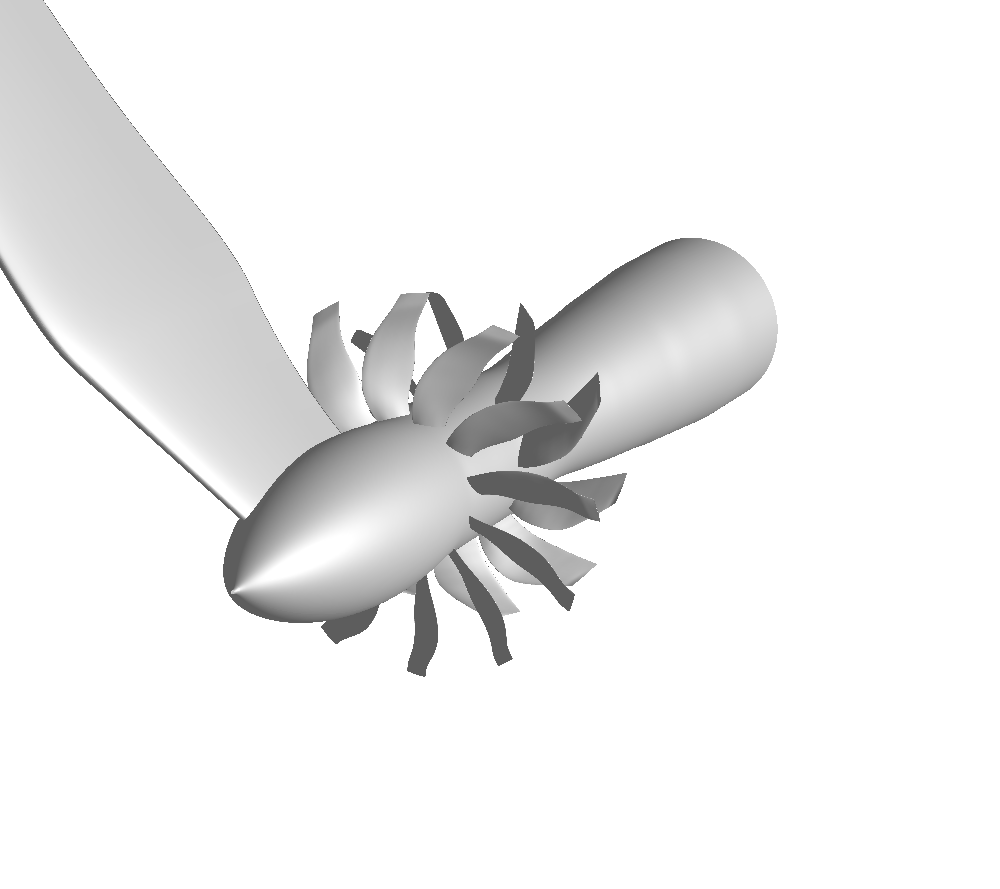
\includegraphics[width=.4\textwidth]{HERA3_INSTALLED_wall.png}}
  \subfigure[prediction tool]{
  	\label{fig:hera3_perspectives}
  	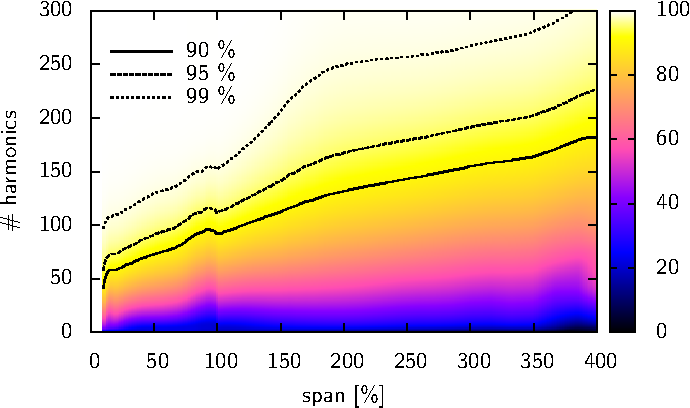
\includegraphics[width=0.40\textwidth]{HERA3_INSTALLED_RANS_SPECTRUM_PPT.pdf}}
  \caption{Number of harmonics required to compute an 
  installed contra-rotating open rotor configuration.}
\end{figure}

For such unsteady signals, the Fourier basis
is not optimal as shown in 
\hyperref[cha:limitations_convergence]{\emph{Chapter~6}}.
\citet{Li2002} propose a wavelet-balance approach to
solve this type of configuration. This
solution sounds promising and should be tested on
wake signals. 

\citet{Ferrante2013} used a multi-frequential Fourier-based time
method to investigate incidence effects on the noise
emission of a CROR. This sort of application is a good candidate
for the multi-frequential HB approach as the full annulus
distortion is more likely to be close to a sine function which
requires few harmonics to be captured. The advantage of the
prediction tool developed in the current work is that
it can be used on any steady computation to \emph{a priori}
estimate the number of harmonics required to simulate the
configuration. As such, it helps choosing whether or not
a Fourier-based time method might be more efficient than
a classical time-marching approach.


\subsection*{On the aeroelasticity of contra-rotating open rotors}

In this work, a numerical approach has been developed to
simulate the aeroelasticity of CROR. Only the flutter of the
front rotor blades has been investigated. The rear rotor
flutter remains to be studied. In addition to that, forced
response simulations are needed to evaluate the vibration
level of the rear rotor blades. The problem is that the
proposed approach relies on a weak-coupling meaning
that the forced response level can not be classically evaluated.
Two solution
